\documentclass[12pt, a4paper]{report}

\usepackage[utf8]{inputenc}
\usepackage{geometry}
 \geometry{
 a4paper,
 total={170mm,257mm},
 left=20mm,
 top=20mm,
}

\usepackage{titlesec}
\titleformat
{\chapter}
[display]{\bfseries\Large\itshape}
{Capitolo Nr.\thechapter}
{0.5ex}
{
    \rule{\textwidth}{1pt}
    \vspace{1ex}
	\centering
}
[\vspace{-0.5ex}\rule{\textwidth}{0.3pt}]
\renewcommand{\contentsname}{Indice}

\usepackage{amssymb,amsmath,amsthm}
\newtheoremstyle{def}
{\topsep}{\topsep}%
{\em}{}%
{\bfseries}{}
{\newline}
{%
  \rule{\textwidth}{0.4pt}\\*%
  \thmname{#1}~\thmnumber{#2}\thmnote{\ -\ #3}.\\*[-1.5ex]%
  \rule{\textwidth}{0.4pt}}%

\theoremstyle{def}
\newtheorem{definition}{Definizione}

\theoremstyle{definition}
\newtheorem*{note}{NB}

\usepackage{graphicx}
\usepackage{subfig}
\usepackage{caption}
\graphicspath{{./images/}}% Imposta il percorso relativo per le immagini
\renewcommand{\figurename}{Fig.}% Cambia il testo delle caption

\title{Dispense di Ingegneria del software}
\author{Leonardo De Faveri}
\date{A.A. 2021/2022}

\begin{document}
\maketitle
\tableofcontents

\chapter{Introduzione}
\section{Definizione e finalità dell'Ingegneria del software}
Iniziamo questa trattazione con una definizione formale di \emph{Ingegneria del
Software} (\emph{IS}):
\begin{definition}[Ingegneria del software]
    L'Ingegneria del software si definisce come:
    \begin{enumerate}
        \item Applicazione di una strategia sistematica, disciplinata e
        misurabile allo sviluppo, esercizio e manutenzione di un software;
        \item Studio delle strategie di cui al punto (1);
    \end{enumerate}
\end{definition}\noindent
L'obiettivo finale dell'\emph{IS} è quindi lo sviluppo di un software di qualità.

\subsection{L'IS come tecnologia}
Per comprendere meglio cosa sia questa disciplina, possiamo immaginarla come una
tecnologia suddivisa in livelli.

\begin{figure}[h]
    \centering
    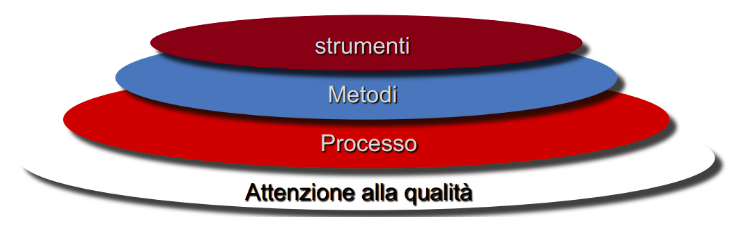
\includegraphics[width=\textwidth]{strati-is.png}
    \caption{Schema degli strati dell'\emph{Ingegneria del software}}
\end{figure}\noindent
Alla base abbiamo l'obiettivo, ovvero lo sviluppo di un prodotto di qualità.
Per fare ciò, esistono diversi \emph{processi} che definiscono e organizzano le
attività da svolgere. Similmente, il modo in cui le attività devono essere svolte
e collegate tra loro, è stabilito dai \emph{metodi}. Infine, per rendere efficiente
il corso delle attività, esistono dei supporti automatizzati detti \emph{strumenti}.
\newpage
\noindent Per rendere più chiaro quanto appena detto possiamo anche dire che:
\begin{itemize}
    \item \emph{Processi}: definiscono e organizzano le attività da svolgere per
    realizzare il prodotto finito;
    \item \emph{Metodi}: indicano come portare a termine le singole attività e
    anche come mettere in relazione attività diverse (e.g. analisi dei requisiti,
    progettazione dell'architettura, scrittura di documentazione);
    \item \emph{Strumenti}: permettono di rendere più efficiente il lavoro
    (e.g. software per lo sviluppo del codice, linguaggi di modellazione, tool
    per il testing, \dots);
\end{itemize}

\chapter{Processi di sviluppo}
\begin{definition}[Processo di sviluppo]
    Un \emph{processo di sviluppo} stabilisce quando e come qualcuno deve fare
    cosa, per raggiungere un obiettivo.
\end{definition}\noindent
Chiaramente, a seconda del progetto, può essere più conveniente seguire un certo
tipo di \emph{processo} invece di un altro. È anche possibile far valutare il
proprio processo di sviluppo, così da garantire ai propri clienti che verranno
mantenuti determinati livelli di qualità.

\section{Modelli per processi di sviluppo}
Vediamo ora una carrellata dei più diffusi \emph{modelli per processi di sviluppo}.
\subsection{Modello a cascata}
Il \emph{modello a cascata}, o \emph{waterfall}, descrive l'approccio classico allo
sviluppo di un software.

Con questo tipo di \emph{processo}, una volta che i requisiti sono noti, il
lavoro procede in maniera lineare e si conclude con la consegna del prodotto
finito al cliente.

\begin{figure}[h]
    \centering
    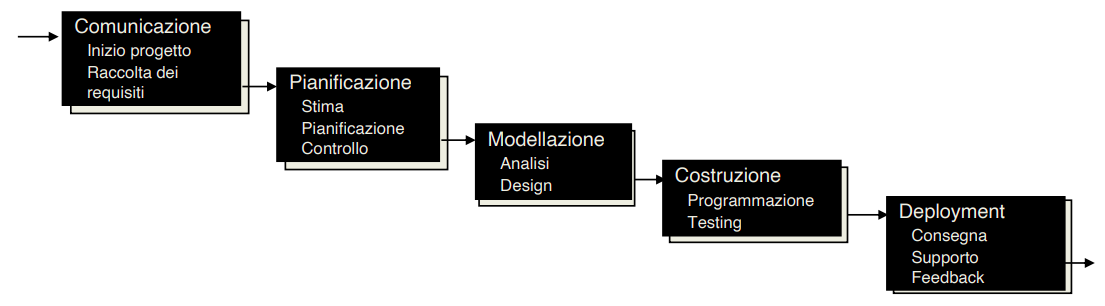
\includegraphics[width=\textwidth]{modello-waterfall.png}
    \caption{Schema del \emph{modello a cascata}}
\end{figure}\noindent
Il problema con questo tipo di approccio è che il mancato coinvolgimento del
cliente (o in generale di parte degli stakeholder) nelle fasi intermedie, porta
la maggior parte dei prodotti a disattendere le richieste del cliente e quindi
al fallimento del progetto. Inoltre, qualora si rendesse necessario una modifica
a quanto fatto in una fase di sviluppo precedente, sarebbe necessario un
impiego di tempo e risorse non indifferente.

Per queste ragioni, il \emph{modello a cascata} non viene più utilizzato, se non
in progetti di dimensioni molto ridotte.

\subsection{Modello incrementale}
Nel \emph{modello incrementale} lo sviluppo del software procede per aggiunta
di funzionalità a una versione base del software. Può essere visto come
uno sviluppo in contemporanea di più \emph{processi con modello a cascata}.

\begin{figure}[h]
    \centering
    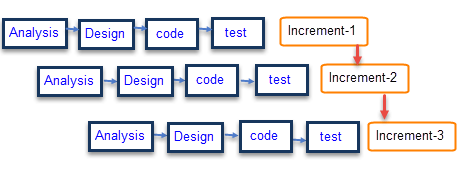
\includegraphics[width=\textwidth]{modello-incrementale.png}
    \caption{Schema del \emph{modello incrementale}}
\end{figure}\noindent
Questo modello argina parzialmente alcuni dei problemi del precedente, in quanto
ogni incremento inizia con il coinvolgimento del cliente e, se le aggiunte sono
minime, si riducono anche i costi in caso di modifiche o errori.

\subsection{Modello a prototipi}
Questo tipo di approccio va bene quando il cliente non ha un'idea chiara del
prodotto che vuole realizzare. Il team di sviluppo produce quindi un prototipo
basandosi sulle poche indicazioni ricevute e lo sottopone al cliente.

Se il cliente valida il prototipo, questo viene fatto evolvere per arrivare a
un prodotto finito, altrimenti si ricomincia con un nuovo prototipo.

\begin{figure}[ht]
    \centering
    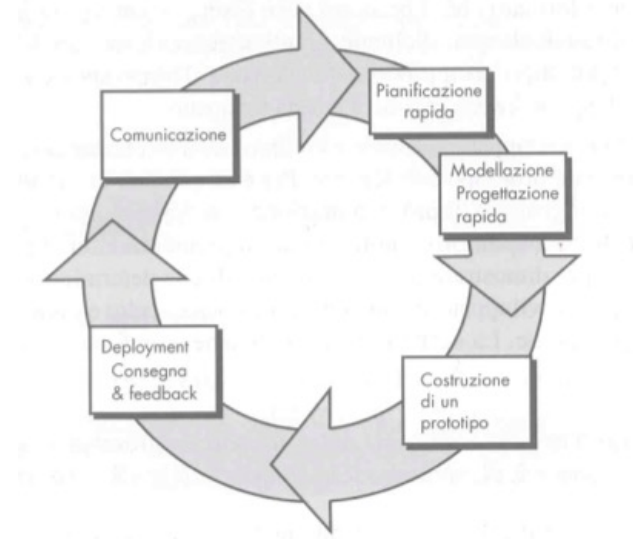
\includegraphics[scale=0.5]{modello-a-prototipi.png}
    \caption{Schema del \emph{modello a prototipi}}
\end{figure}

\paragraph{Prototipo}
\begin{definition}[Prototipo]
    Un \emph{prototipo} è una rappresentazione di un prodotto o di un sistema, o
    di una sua parte, che, anche se in qualche modo limitata, può essere
    utilizzata a scopo di valutazione.
\end{definition}

Il \emph{prototipo} non deve necessariamente essere un prodotto funzionante,
può anche essere un modello "finto" che dia soltanto un'idea di quali potrebbero
essere le funzionalità e il \emph{look and feel} del prodotto finito.

Per realizzare il prodotto finito è meglio non partire dal prototipo, in quanto,
spesso, nel suo sviluppo, si sono sacrificati gli aspetti relativi alla qualità
per prediligere invece la velocità di realizzazione. È quindi preferibile
ricominciare lo sviluppo usando il \emph{prototipo} come riferimento per le
funzionalità e le caratteristiche da implementare.

\paragraph{Wireframe o mock-up}
Come detto il \emph{prototipo} non deve necessariamente essere un qualcosa di
funzionante, ma può limitarsi a dare un'idea delle funzioni e dall'aspetto del
prodotto finito. In questo contesto, si inseriscono due strumenti: i
\emph{wireframe} e i \emph{mock-up}.
\begin{itemize}
    \item \emph{Wireframe}: permette di capire quale sarà l'esperienza utente,
    la cosiddetta \emph{user experience}. Si tratta di una bozza grafica,
    fatta anche su carta, priva di tutti gli elementi di design, cioè mancano
    colori, immagini e quant'altro;
    \item \emph{Mock-up}: contiene gli elementi di design e serve a dimostrare
    quello che potrebbe essere il \emph{look and feel} del prodotto;
\end{itemize}

\begin{figure}[h]
    \centering
    \subfloat[\emph{Wireframe}]{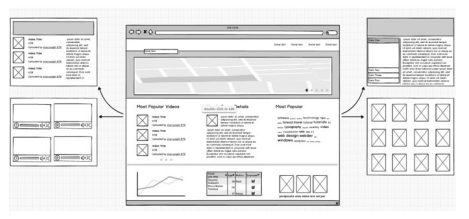
\includegraphics[scale=0.62]{wireframe.png}}
    \hfill
    \subfloat[\emph{Mock-up}]{
\includegraphics[scale=0.62]{mock-up.png}}
    \caption{\emph{Wireframe} e \emph{mock-up}}
\end{figure}

\newpage
\subsection{Modello a spirale}
Nel \emph{modello a spirale} si segue approccio iterativo: ad ogni "giro" viene
consegnata una versione del prodotto. Questo è simile a quanto avviene nel
\emph{modello incrementale}, ma mentre nel \emph{modello incrementale} si
costruisce su di una versione base, qui è sempre possibile ricominciare da capo.
Spesso, infatti, si inizia con dei prototipi e quando un prototipo soddisfa le
richieste del cliente si procede con lo sviluppo del prodotto vero e proprio.

Si può dire che questo approccio unisca l'iteratività del \emph{modello a
prototipi} alla \emph{sistematicità} di quello a \emph{cascata}.

\begin{figure}[h]
    \centering
    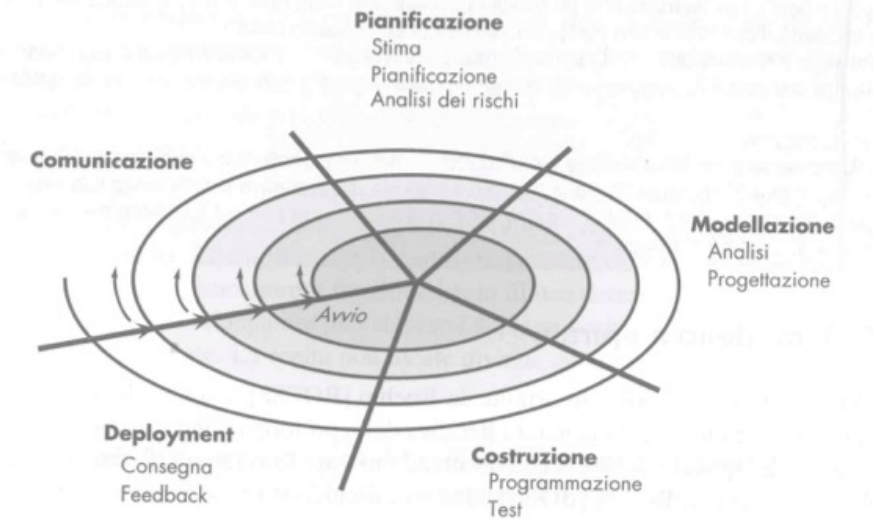
\includegraphics[width=\textwidth]{modello-a-spirale.png}
    \caption{Schema del \emph{modello a spirale}}
\end{figure}

\subsection{Modello di sviluppo a componenti}
Vengono realizzati componenti software con funzionalità e interfacce ben
definite. I singoli componenti vengono poi collegati per realizzare il
prodotto finale.

\begin{figure}[h]
    \centering
    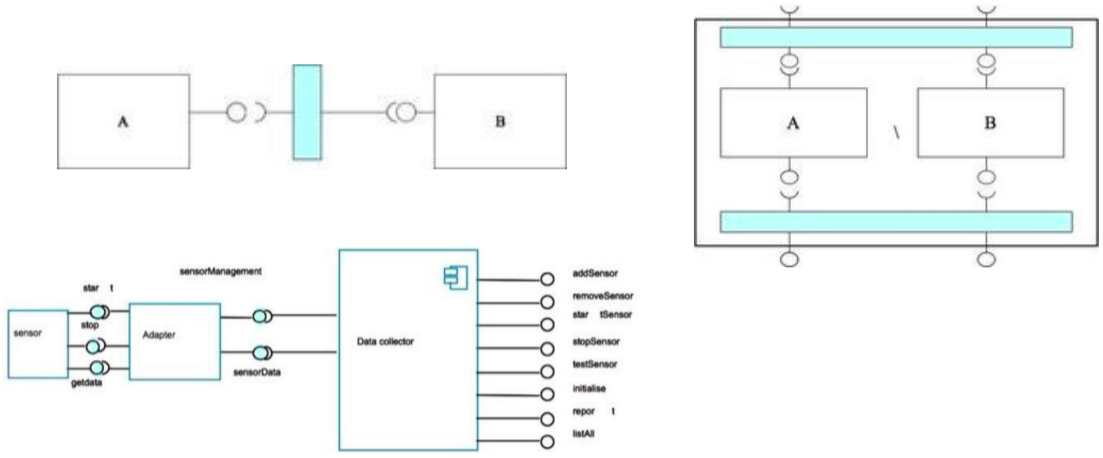
\includegraphics[scale=0.33]{modello-a-componenti.png}
    \caption{Schema del \emph{modello di sviluppo a componenti}}
\end{figure}\noindent
Questo approccio permette di dividere facilmente il lavoro in problemi più
semplici e contemporaneamente di ridurre i costi per eventuali interventi
correttivi o aggiunte. Tuttavia, spesso è necessario produrre del codice
ausiliario detto \emph{glue-code} per consentire i componenti di comunicare
correttamente tra loro.

\paragraph{Architetture orientate ai servizi}
La \emph{Service Oriented Architecture} (\emph{SOA}) è il modello che sta alla
base di particolari architetture, oggi sempre più diffuse, che si basano proprio
sullo sviluppo di servizi distribuiti e indipendenti tra loro che vengono poi
combinati per realizzare software complessi. I vantaggi di questo tipo di
architetture sono la scalabilità e la modularità, che vengono favorite proprio
dall'indipendenza dei singoli servizi.

Uno esempio di questo è l'\emph{architettura a microservizi}, o \emph{Microservices
Architecture} (\emph{MA}), nella quale componenti con funzionalità minime
vengono combinate per realizzare software complessi. Questo tipo di sviluppo è
particolarmente adatto per applicazioni che hanno la necessità di scalare ed
evolversi rapidamente soprattutto sfruttando il cloud.

\subsection{Model-driven developement}
Secondo questo approccio, lo sviluppo del prodotto procede di pari passo con la
modellazione del sistema software: i modelli evolvono con il procedere dello
sviluppo. Si parte cioè, con la creazione di un modello dell'architettura nel
suo insieme e, mano a mano che il lavoro procede, vengono aggiunte alla
rappresentazione le descrizioni di componenti più specifici. Di conseguenza, il
livello di dettaglio del modello andrà ad aumentare progressivamente.

Esistono linguaggi e strumenti appositi che permettono sia di definire i
modelli che di implementarli in codice.

\section{Metodologie agili}
Esistono modelli di sviluppo cosiddetti \emph{agili}, o \emph{agile}, che propongono
paradigmi il cui focus è sull'interazione col cliente piuttosto che sul prodotto.
Nelle \emph{metodologie agili} infatti, il processo di sviluppo del software
cerca di coinvolgere quanto più possibile il cliente, ottenendo in questo modo
un prodotto maggiormente conforme alle sue richieste.

Proprio questa caratteristica fa si che i progetti realizzati in questo modo
abbiano un tasso di successo molto superiore rispetto a quelli che usano il
classico \emph{modello a cascata}.

Non bisogna erroneamente pensare che i \emph{processi agili} siano totalmente
contrapposti ai modelli più tradizionali. Infatti, molti dei concetti di queste
metodologie sono adattamenti dei migliori concetti dell'\emph{ingegneria del
software} tradizionale. Ad esempio, viene mantenuta l'iteratività caratteristica
del \emph{modello incrementale}.

\subsection{Modello scrum}
Il \emph{modello scrum} (mischia) è un insieme di pratiche e regole che consentono
di ridurre l'overhead amministrativo. In particolare, il lavoro viene diviso in
task che sono assegnati a piccoli gruppi di lavoro, tipicamente di 3-4 componenti.
Ogni team ha molta libertà nell'organizzazione del proprio lavoro e nella
distribuzione delle responsabilità tra i propri componenti, ad esempio nella
scelta del proprio responsabile.

Lo sviluppo del software procede poi in maniera incrementale e con attività
continue di testing e manutenzione.

Interessante è il modo in cui è organizzato il progetto nel suo insieme: il
progetto viene diviso in blocchi rapidi di lavoro detti \emph{sprint} alla fine
dei quali viene consegnata al cliente una versione del software. Vengono inoltre
svolte giornalmente riunioni dei singoli team di sviluppo, dette \emph{daily scrum}
nelle quali ci si confronta sul lavoro svolto e quello rimanente. Il \emph{modello
scrum} prevede anche che vengano definiti i \emph{backlog}, cioè i dettagli del
lavoro da fare nell'immediato futuro. Questo permette di avere una visione estesa
dello stato del progetto.

\begin{figure}[t]
    \centering
    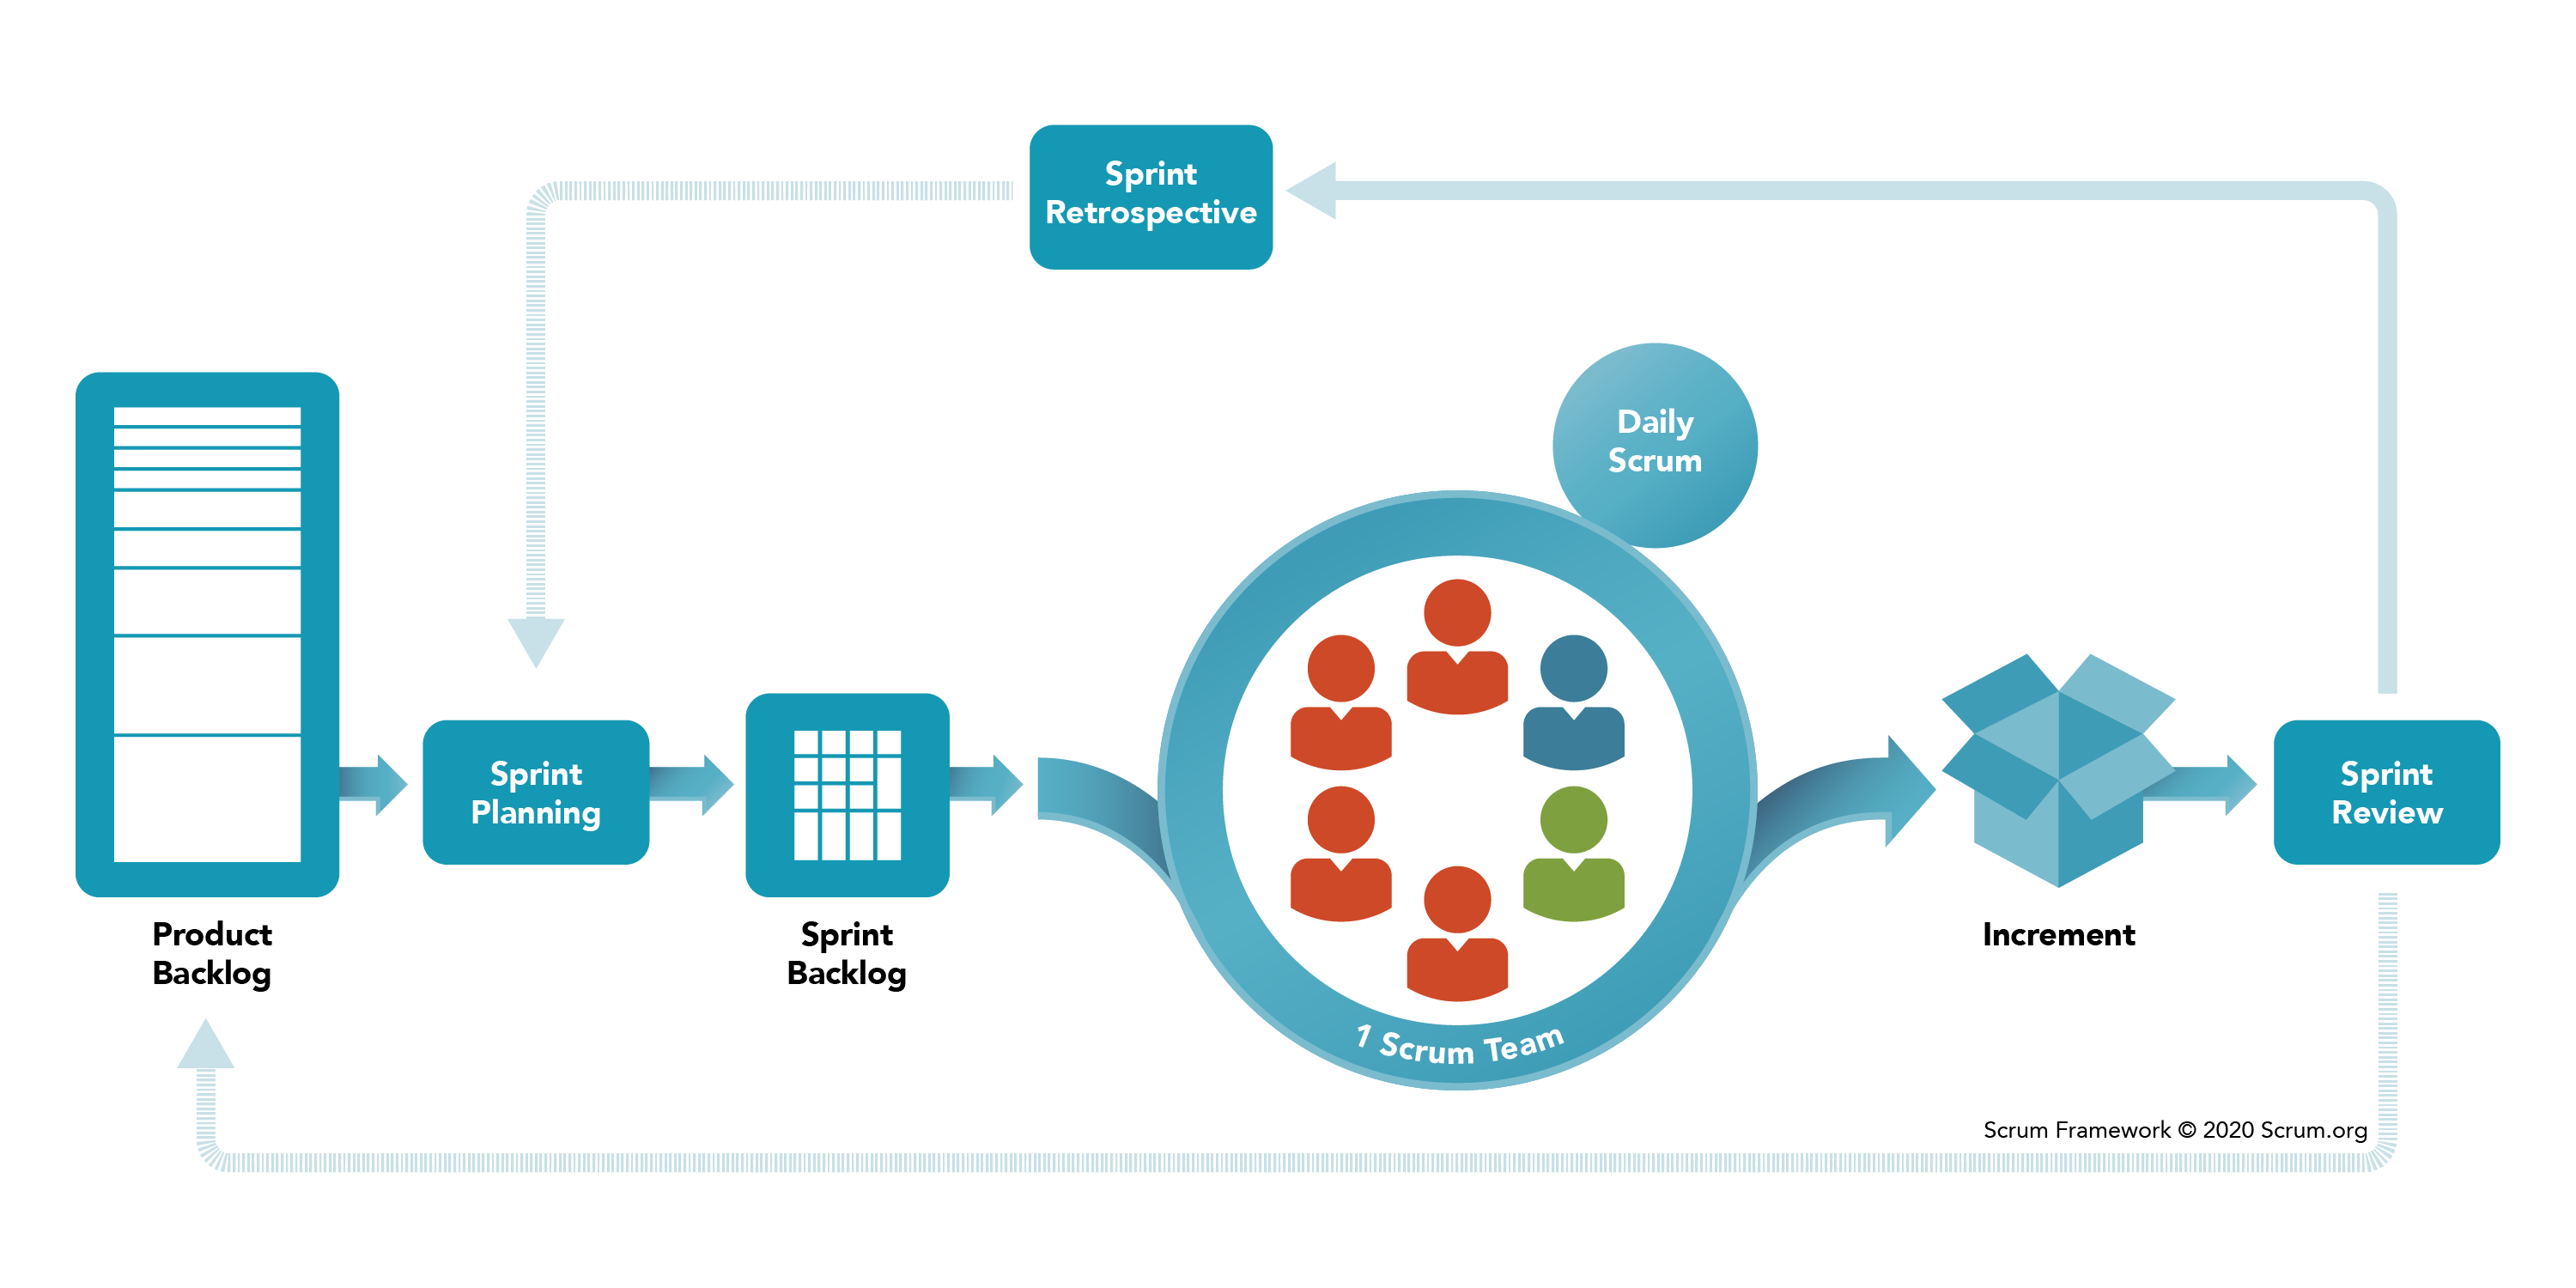
\includegraphics[width=\textwidth]{modello-scrum.png}
    \caption{Schema del \emph{modello scrum}}
\end{figure}

\subsection{Modello extreme programming}
Questa metodologia ha un approccio \emph{object-oriented} allo sviluppo ed è
caratterizzata da 4 valori e 12 pratiche. I valori sono:
\begin{enumerate}
    \item \emph{Semplicità};
    \item \emph{Comunicazione};
    \item \emph{Testing};
    \item \emph{Coraggio};
\end{enumerate}
Le 12 pratiche possono invece essere raggruppate in 4 aree fondamentali:
\begin{enumerate}
    \item \emph{Feedback a scala fine}: la consegna del software avviene
    tramite frequenti rilasci che incrementano anche in minima parte le
    funzionalità del prodotto;
    \item \emph{Processo continuo}: l'integrazione delle modifiche nel sistema
    viene fatta frequentemente, così da limitare eventuali conflitti con il
    codice esistente. Questo tipo di processo è strettamente sequenziale, cioè
    un solo programmatore alla volta integra le proprio modifiche, testa e
    rilascia il software;
    \item \emph{Comprensione condivisa}: la pianificazione del lavoro è basata
    su un insieme di \emph{user story} definite dal cliente;
    \item \emph{Benessere dei programmatori}: il codice viene modificato, anche
    nella sua architettura, per migliorarne le prestazioni e la comprensibilità;
\end{enumerate}
\paragraph{Pianificazione a user story}
All'avvio del progetto, il cliente fornisce al team di sviluppo (nel suo intero
o un gruppo specifico) una descrizione delle funzionalità e delle caratteristiche
che dovrà avere il software. Questa descrizione di insieme viene suddivisa in
componenti più semplici detti \emph{user story}.

A ogni \emph{user story} il cliente assegna un valore, in modo che venga data
priorità alle \emph{user story} col valore più alto. Il team di sviluppo valuta
le \emph{user story} e a ciascuna assegna un costo, descritto come tempo di
sviluppo. Se il costo è troppo alto, viene chiesto al cliente di spezzare la
\emph{user story} in casi più semplici.

In fase di sviluppo il team può decidere come implementare le \emph{user story}
(in ordine di priorità, in ordine di costo, tutte insieme, \dots), ciò che importa
è che vengano concordate con il cliente le date di rilascio e quali
\emph{user story} dovranno essere incluse in ogni release.

\paragraph{Approccio al testing}
L'\emph{Extreme Programming} stabilisce anche un approccio al testing. Vengono
implementati degli \emph{Unit test} che vanno a convalidare il funzionamento di
ciascuna \emph{user story}. I test non valutano l'implementazione complessiva
delle \emph{user story}, ma si assicurano soltanto che a ogni input corrisponda
un output corretto.

Questa caratteristica permette agli sviluppatori di concentrarsi in prima battuta
soltanto sull'aspetto \emph{estensionale} del codice. Grazie a ciò, il tempo di
rilascio della prima versione viene ridotto. Future attività di \emph{refactoring}
andranno a migliorare l'aspetto \emph{intensionale} del codice e l'efficienza
complessiva delle release successive.

L'attività di testing può essere automatizzata mediante l'utilizzo di
\emph{testing suite universali} col risultato che \emph{integration} e
\emph{validation test} possono essere eseguiti quotidianamente. I cosiddetti
\emph{acceptance test}, o \emph{customer test}, cioè l'attività di verifica
dell'utente finale diventano quindi più semplici, in quanto si possono
concentrare soltanto sulle funzioni e le caratteristiche globali del sistema.

\paragraph{Pair programming}
La programmazione avviene in coppia, cioè a ogni workstation lavorano due
programmatori. Questo garantisce una maggiore qualità del software prodotto,
perché vi è sempre un controllore e, inoltre, semplifica e velocizza la
risoluzione dei problemi.

\subsection{DevOps}
Una figura che sta assumendo maggiore importanza nelle grandi aziende e quella
del \emph{DevOps} (\emph{Developement + Operations}). In ambienti strutturati e
complessi i componenti software vengono installati su infrastrutture altrettanto
complesse. Il compito del \emph{DevOps} è quello di coordinare il lavoro di
sviluppo software con quello di manutenzione dell'infrastruttura, in modo da
efficientare questa interazione e ridurre l'insorgere di problemi.

\chapter{Linguaggi di modellazione}
Nello sviluppo di un software, prima di passare all'implementazione vera e
propria, è consigliabile ragionare su una versione semplificata della realtà
che si vuole realizzare. Tale visione semplificata è detta \emph{modello}.

\begin{definition}[Modello]
    Un \emph{modello} è la rappresentazione semplificata di un'entità. Sono
    presenti solo le informazioni importanti e astrazioni dei concetti più
    complessi.
\end{definition}\noindent
Un buon \emph{modello}, oltre che rappresentare in modo semplice la realtà, deve
anche poter essere compreso da soggetti terzi rispetto ai suoi creatori. Cioè, è
necessario che venga creato usando un linguaggio standardizzato e diffuso.

Nell'\emph{ingegneria del software} esistono diversi linguaggi a seconda di ciò
che si vuole rappresentare ed è quindi importante saper scegliere quello corretto.
Tra le caratteristiche di un buon linguaggio vanno considerate:
\begin{itemize}
    \item \emph{Semplicità di utilizzo}: deve consentire di esprimersi con
    facilità e contemporaneamente deve essere di facile comprensione;
    \item \emph{Fruibilità diffusa}: deve poter essere compreso anche da soggetti
    non esperti in materia;
    \item \emph{Formalità}: un linguaggio formale e preciso può essere usato per
    descrivere realtà e concetti complessi senza ambiguità e a livelli d'astrazione
    diversi;
\end{itemize}
Alcuni esempi di linguaggi di modellazione sono il linguaggio
\emph{Entity-Relationship} per la progettazione concettuale di database, il
\emph{BPMN} (\emph{Business Process Modelling Notation}) per la rappresentazione dei
processi di business.

\section{Modellare i requisiti di sicurezza}
Nella realizzazione di un software di qualità non si può non considerare
l'aspetto della sicurezza. La definizione dei requisiti di sicurezza può
essere realizzata con diversi linguaggi. Questo tipo di linguaggi rientra nella
definizione di \emph{Security Requirements Engineering} (\emph{SRE}).

\subsection{Misuse-case diagram}
Questo linguaggio è basato sulla sintassi \emph{UML} (\emph{Unified Modeling
Language}) e consente di rappresentare i casi d'uso improprio del software.
Cioè, consente di descrivere quali utilizzi (percorsi di utilizzo) del software
potrebbero avere conseguenze sgradite. Visualizzare questi percorsi permette
all'ingegnere del software di progettare un'architettura che li neutralizzi.

\begin{figure}[h]
    \centering
    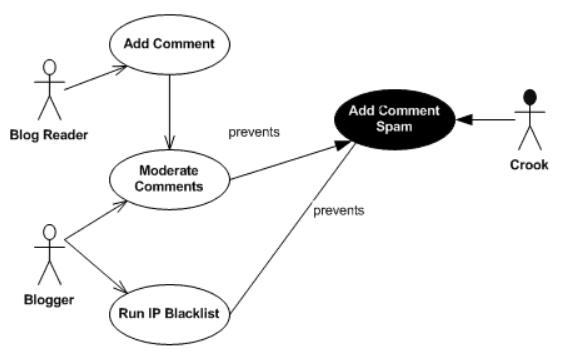
\includegraphics[width=\textwidth]{misuse-case-diagram.png}
    \caption{Esempio di \emph{misuse-case diagram}}
\end{figure}

\subsection{Linguaggi goal-oriented}
Alcuni linguaggi si concentrano invece sull'ipotizzare quali potrebbero essere
gli obiettivi di utenti malintenzionati, i cosiddetti \emph{anti-goal}, così da
poter poi a progettare il software in modo che quegli obiettivi non siano
realizzabili.

\section{Linguaggio UML}
L'\emph{UML} è certamente il linguaggio più usato nell'\emph{ingegneria del
software}. Grazie ai suoi dialetti può essere usato per modellare diversi
aspetti di un software. Gli ambiti d'uso dell'\emph{UML} sono:
\begin{itemize}
    \item \emph{Use-case diagram}: letteralmente il \emph{diagramma dei casi
    d'uso}, rappresenta cioè quello che ci si aspetta possa fare l'utente;
    \item \emph{Activity diagram}: descrive come ci si aspetta che vengano svolte
    le singole attività;
    \item \emph{Sequene diagram}: descrive in modo sequenziale l'interazione tra
    due oggetti;
    \item \emph{Class diagram}: consente di definire la struttura di una o più
    classi nell'ambito della OOP;
    \item \emph{Deploy diagram}: raffigura i requisiti e i passi da compiere per
    il rilascio del software;
\end{itemize}

\paragraph{Activity diagram VS Sequence diagram}
Questi due diagrammi potrebbero sembrare simili, ma in realtà hanno una differenza
piuttosto marcata.

\begin{figure}[th]
    \centering
    \subfloat[\emph{Activity diagram}]{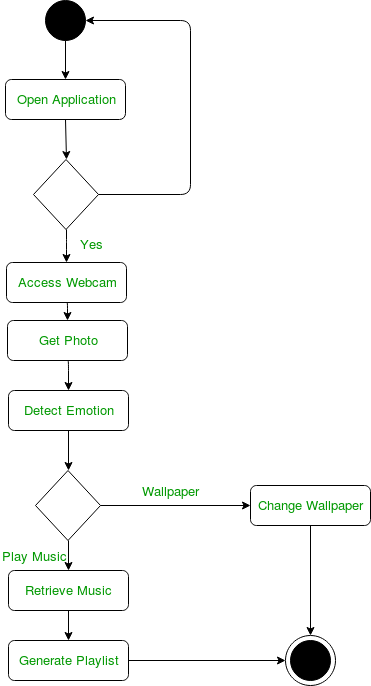
\includegraphics[scale=0.56]{activity-diagram-exampe.png}}
    \hfill
    \subfloat[\emph{Sequence diagram}]{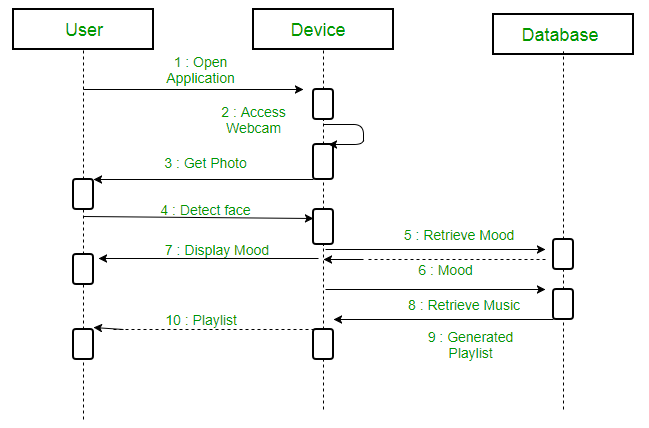
\includegraphics[scale=0.56]{sequence-diagram-example.png}}
    \caption{\emph{Activity diagram} VS \emph{Sequence diagram}}
\end{figure}\noindent
Come si può vedere l'\emph{activity diagram} descrive il flusso delle operazioni
necessarie per passare da un'attività a un'altra, mentre il \emph{sequence
diagram} descrive lo scambio di messaggi tra un oggetto e un altro.

Si può comprendere meglio la differenza tra i due se si vede l'\emph{activity
diagram} come un \emph{diagramma di flusso} e il \emph{sequence diagram} come
il diagramma descrittivo di un evento.

\subsection{Linguaggio OCL}
L'\emph{OCL} (\emph{Object Constraint Language}) è una versione estesa di
\emph{UML}. È un linguaggio funzionale e consente di rappresentare vincoli ed
espressioni in modelli \emph{object-oriented}.

\chapter{Requisiti}
\section{Requisiti non funzionali}
I requisiti non funzionali definiscono le proprietà che deve avere il prodotto
realizzato.

\end{document}
